
\chapter{Registration}

\itkpiccaption[Image Registration Concept]{Image registration is the task of
finding a spatial transform mapping on image into
another.\label{fig:ImageRegistrationConcept}}
\parpic(8cm,3cm)[r]{\includegraphics[width=8cm]{ImageRegistrationConcept.eps}}
  
This chapter introduces ITK's capabilities for performing image
registration. Image registration is the process of determining the spatial
transform that maps points from one image to homologous points on a object in
the second image. This concept is schematically represented in Figure
\ref{fig:ImageRegistrationConcept}. In ITK, registration is performed within
a framework of pluggable components that can easily be interchanged.  This
flexibility means that a combinatorial variety of registration methods can be
created, allowing users to pick and choose the right tools for their specific
application.


\section{Registration Framework}
The components of the registration framework and their interconnections are
shown in Figure \ref{fig:RegistrationComponents}. The basic input data to the
registration process are two images: one is defined as the \emph{fixed} image
$f(\bf{X})$ and the other as the \emph{moving} image $m(\bf{X})$. Where
$\bf{X}$ represents a position in N-dimensional space. Registration is treated
as an optimization problem with the goal of finding the spatial mapping that
will bring the moving image into alignment with the fixed image.

\begin{figure}
\center
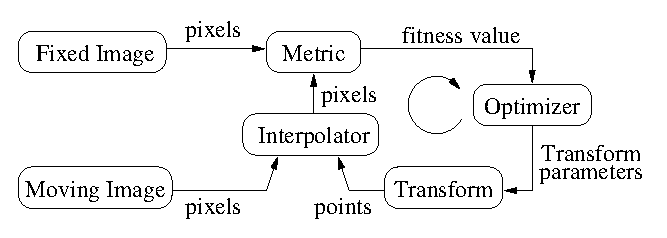
\includegraphics[width=0.8\textwidth]{RegistrationComponentsDiagram.eps}
\itkcaption[Registration Framework Components]{The basic components of the
registration framework are two input images, a transform, a metric, an
interpolator and an optimizer.}
\label{fig:RegistrationComponents}
\end{figure}

The \emph{transform} component $T(\bf{X})$ represents the spatial mapping of
points from the fixed image space to points in the moving image space. The
\emph{interpolator} is used to evaluate moving image intensities at non-grid
positions. The \emph{metric} component $S(f,m \circ T)$ provides a measure of
how well the fixed image is matched by the transformed moving image. This
measure forms the quantitative criterion to be optimized by the
\emph{optimizer} over the search space defined by the parameters of the
\emph{transform}.

These various ITK registration components will be described in later
sections.  First, we begin with some simple registration examples.

\section{"Hello World" Registration}
\label{sec:IntroductionImageRegistration}
\ifitkFullVersion
\input{ImageRegistration1.tex}
\fi

\section{Features of the Registration Framework}
\label{sec:FeaturesOfTheRegistrationFramework}

\begin{figure}
\center
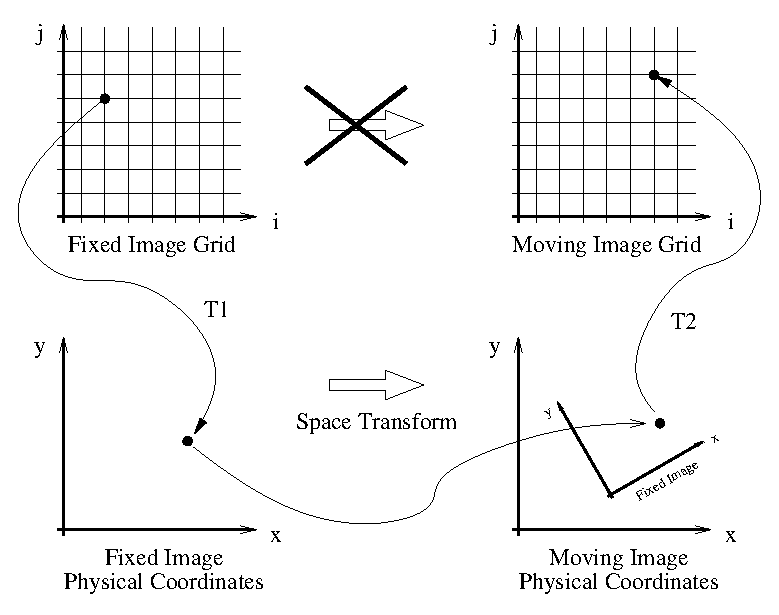
\includegraphics[width=0.75\textwidth]{ImageRegistrationCoordinateSystemsDiagram.eps}
\itkcaption[Registration Coordinate Systems]{Different coordinate systems
involved in the image registration process. Note that the transform being
optimized is the one mapping from the physical space of the fixed image
into the physical space of the moving image.}
\label{fig:ImageRegistrationCoordinateSystemsDiagram}
\end{figure}


This section presents a discussion on the two most common difficulties that
users encounter when they start using the ITK registration framework. They are,
in order of difficulty

\begin{itemize}
\item The direction of the Transform mapping
\item The fact that registration is done in physical coordinates
\end{itemize}

Probably the reason why these two topics tend to create confusion is that they
are implemented in different ways in other systems and therefore users tend to
have different expectations regarding how things should work in ITK. The
situation is further complicated by the fact that most people describe image
operations as if they were manually performed in a picture in paper.

\subsection{Direction of the Transform Mapping}
\label{sec:DirectionOfTheTransformMapping}

The Transform that is optimized in the ITK registration framework is the one
that maps points from the physical space of the fixed image into the physical
space of the moving image. This is illustrated in
Figure~\ref{fig:ImageRegistrationCoordinateSystemsDiagram}. This implies that
the Transform will accept as input points from the fixed image and it will
compute the coordinates of the analogous points in the moving image. What tends
to create confusion is the fact that when the Transform shifts a point on the
\textbf{positive} X direction, the visual effect of this mapping, once the
moving image is resampled, is equivalent to {\em manually shifting} the moving
image along the \textbf{negative} X direction. In the same way, when the
Transform applies a \textbf{clock-wise} rotation to the fixed image points, the
visual effect of this mapping once the moving image has been resampled is
equivalent to {\em manually rotating} the moving image
\textbf{counter-clock-wise}. 

The reason why this direction of mapping has been chosen for the ITK
implementation of the registration framework is that this is the direction that
better fits the fact that the moving image is expected to be resampled using
the grid of the fixed image. The nature of the resampling process is such that
an algorithm must go through every pixel of the {\em fixed} image and compute
the intensity that should be assigned to this pixel from the mapping of the
{\em moving} image. This computation involves taking the integral coordinates
of the pixel in the image grid, usually called the ``(i,j)'' coordinates,
mapping them into the physical space of the fixed image (transform \textbf{T1}
in Figure~\ref{fig:ImageRegistrationCoordinateSystemsDiagram}), mapping those
physical coordinates into the physical space of the moving image (Transform to
be optimized), then mapping the physical coordinates of the moving image in to
the integral coordinates of the discrete grid of the moving image (transform
\textbf{T2} in the figure), where the value of the pixel intensity will be
computed by interpolation. 

If we have used the Transform that maps coordinates from the moving image
physical space into the fixed image physical space, then the resampling process
could not guarantee that every pixel in the grid of the fixed image was going
to receive one and only one value. In other words, the resampling will have
resulted in an image with holes and with redundant or overlapped pixel values.

As you have seen in the previous examples, and you will corroborate in the
remaining examples in this chapter, the Transform computed by the registration
framework is the Transform that can be used directly in the resampling filter
in order to map the moving image into the discrete grid of the fixed image.

There are exceptional cases in which the transform that you want is actually
the inverse transform of the one computed by the ITK registration framework.
Only in those cases you may have to recur to invoking the \code{GetInverse()}
method that most transform offer.  Make sure that before you consider following
that dark path, you interact with the examples of resampling illustrated in
section~\ref{sec:GeometricalTransformationFilters} in order to get familiar
with the correct interpretation of the transforms.


\subsection{Registration is done in physical space}
\label{sec:RegistrationIsDoneInPhysicalSpace}

The second common difficulty that users encounter with the ITK registration
framework is related to the fact that ITK performs registration in the context
of physical space and not in the discrete space of the image grid.
Figure~\ref{fig:ImageRegistrationCoordinateSystemsDiagram} show this concept by
crossing the transform that goes between the two image grids. One important
consequence of this fact is that having the correct image origin and image
pixel size is fundamental for the success of the registration process in ITK.
Users must make sure that they provide correct values for the origin and
spacing of both the fixed and moving images.

A typical case that helps to understand this issue, is to consider the
registration of two images where one has a pixel size different from the other.
For example, a PET\footnote{Positron Emission Tomography} image and a
CT\footnote{Computer Tomography in X-rays} image. Typically a CT image will
have a pixel size in the order of 1 millimeter, while a PET image will have a
pixel size in the order of 5 millimeters to 1 centimeter. Therefore, the CT
will need about 500 pixels in order to cover the extent across a human brain, while
the PET image will only have about 50 pixels for covering the same physical
extent of a human brain. 

A user performing registration between a PET image and a CT image may be
naively expecting that because the PET image has less pixels, a {\em scaling}
factor is required in the Transform in order to map this image into the CT
image. At that point, this person is attempting to interpret the registration
process directly between the two image grids, or in {\em pixel space}. What ITK
will do in this case is to take into account the pixel size that the user has
provided and it will use that pixel size in order to compute a scaling factor
for Transforms {\em T1} and {\em T2} in
Figure~\ref{fig:ImageRegistrationCoordinateSystemsDiagram}. Since these two
transforms take care of the required scaling factor, the spatial Transform to
be computed during the registration process does not need to be concerned about
such scaling. The transform that ITK is computing is the one that will
physically map the brain from the moving image into the brain of the fixed
image.

In order to better understand this concepts, it is very useful to draw sketches
of the fixed and moving image {\em at scale} in the same physical coordinate
system. That is the geometrical configuration that the ITK registration
framework uses as context. Keeping this in mind helps a lot for interpreting
correctly the results of a registration process performed with ITK.

\section{Monitoring Registration}
\label{sec:MonitoringImageRegistration}
\ifitkFullVersion
\input{ImageRegistration3.tex}
\fi



\section{Multi-Modality Registration}
\label{sec:MultiModalityRegistration}

Some of the most challenging cases of image registration arise when images of
different modalities are involved. In such cases, metrics based on direct
comparison of gray levels are not applicable. It has been extensively shown
that metrics based on the evaluation of mutual information are well suited for
overcoming the difficulties of multi-modality registration.

\index{itk::Image\-Registration\-Method!Multi-Modality}

The concept of Mutual Information is derived from Information Theory and its
application to image registration has been proposed in different forms by
different groups \cite{Collignon1995,Maes97,Viola1997}, a more detailed review
can be found in \cite{Hajnal2001,Pluim2003}. The Insight Toolkit currently
provides five different implementations of Mutual Information metrics. The
following examples illustrate the practical use of some of these metrics.

\subsection{Viola-Wells Mutual Information}
\label{sec:MultiModalityRegistrationViolaWells}
\ifitkFullVersion
\input{ImageRegistration2.tex}
\fi

\subsection{Mattes Mutual Information}
\label{sec:MultiModalityRegistrationMattes}
\ifitkFullVersion
\input{ImageRegistration4.tex}
\fi


\subsection{Plotting joint histograms}
\label{sec:JointHistograms}
\ifitkFullVersion
\input{ImageRegistrationHistogramPlotter.tex}


\section{ Centered Transforms }

The ITK image coordinate origin is typically located in one of the image
corners. This results in counter-intuitive transform behavior when
rotations and scaling are involved. Users tend to assume that rotations and
scaling are performed around a fixed point at the center of the image.  In
order to compensate for this difference in natural interpretation, a set of
\emph{centered} transforms have been introduced into the toolkit. The following
sections describe the main characteristics of such transforms.

\subsection{Rigid Registration in 2D}
\label{sec:RigidRegistrationIn2D}
\ifitkFullVersion
\input{ImageRegistration5.tex}
\fi

\subsection{Initializing with Image Moments}
\label{sec:InitializingRegistrationWithMoments}
\ifitkFullVersion
\input{ImageRegistration6.tex}
\fi



%\subsection{Similarity Transform in 2D}
%\label{sec:SimilarityRegistrationIn2D}
%\ifitkFullVersion
%\input{ImageRegistration7.tex}
%\fi



\subsection{Rigid Transform in 3D}
\label{sec:RigidRegistrationIn3D}
\ifitkFullVersion
\input{ImageRegistration8.tex}
\fi




\subsection{Centered Affine Transform}
\label{sec:CenteredAffineTransform}
\ifitkFullVersion
\input{ImageRegistration9.tex}
\fi




\section{Multi-Resolution Registration}
\label{sec:MultiResolutionRegistration}
Performing image registration using a multi-resolution approach is widely used
to improve speed, accuracy and robustness. The basic idea is that registration
is first performed at a coarse scale where the images have fewer pixels.
The spatial mapping determined at the coarse level is then used to initialize
registration at the next finer scale. This process is repeated until it
reaches the finest possible scale. This coarse-to-fine strategy greatly
improve the registration success rate and also increases robustness
by eliminating local optima at coarser scales.

The Insight Toolkit offers a multi-resolution registration framework that is
directly compatible with all the registration framework components. The
multi-resolution registration framework has two additional components: a pair
of \emph{image pyramids} that are used to down-sample the fixed and moving
images as illustrated in Figure \ref{fig:MultiResRegistrationComponents}.
The pyramids smooth and subsample the images according to user-defined
scheduling of shrink factors.
 
\begin{figure}
\center
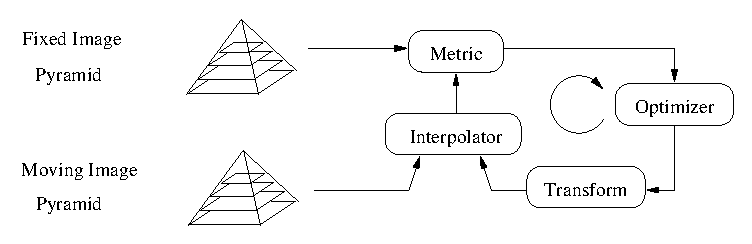
\includegraphics[width=0.8\textwidth]{MultiResRegistrationComponents.eps}
\itkcaption[Multi-Resolution Registration Components]{Components of the
multi-resolution registration framework.}
\label{fig:MultiResRegistrationComponents}
\end{figure}
 
We now present the main capabilities of the multi-resolution framework by
way of an example.

\subsection{Fundamentals}
\ifitkFullVersion
\input{MultiResImageRegistration1.tex}
\fi

\subsection{Parameter Tuning}
\ifitkFullVersion
\input{MultiResImageRegistration2.tex}
\fi

With the completion of these examples, we will now review the main
features of the components forming the registration framework.

\section{Transforms}
\label{sec:Transforms}
\ifitkFullVersion
In the toolkit, \code{itk::Transform} objects encapsulates the mapping of
points, vectors and covariant vectors from an input space to an output space.
The distinction between points, vectors and covariant vectors has already
been discussed in Chapter \ref{sec:DataRepresentation}. If a transform is
invertible, back transform methods are also provided. Currently, 
ITK provide a variety of transfroms from simple translation, rotation and 
scaling to general affine and kernel transforms. Note that, although we
discuss transforms in context registration in this section, transforms
are general and can used for other applications. Some of the commonly used 
transforms will be discussed in detail later in this section.

Typically, each transform type several methods are provided for setting
the parameters. For example, \code{Euler2DTransform} provide methods for
separatedly setting the offset, the angle, and the entire rotation matrix.
However, for use in the registration framework, the parameters must also
be represented by a flat \code{Array<double>} to allow communication
with generic optimizers. In the case of \code{Euler2DTransform}, the transform
is also defined by three doubles: the first representing the angle and 
the last two the offset. The a description of the parameters and their
ordering is documented in the header file of each transform.

Another requirement of the registration framework is the of the
transformation Jacobian. In general, metrics require the knowledge of 
the Jacobian in order to compute the metric derivatives. 
The Jacobian is a matrix whose element are the partial derivatives of the 
output point with respect to the array of parameters that defines the 
transform:

\begin{equation}
J=\left[ \begin{array}{cccc}
\frac{\partial x_{1}}{\partial p_{1}} & 
\frac{\partial x_{2}}{\partial p_{1}} & 
\cdots  & \frac{\partial x_{n}}{\partial p_{1}}\\
\frac{\partial x_{1}}{\partial p_{2}} & 
\frac{\partial x_{2}}{\partial p_{2}} & 
\cdots  & \frac{\partial x_{n}}{\partial p_{2}}\\
\vdots  & \vdots  & \ddots  & \vdots \\
\frac{\partial x_{1}}{\partial p_{m}} & 
\frac{\partial x_{2}}{\partial p_{m}} & 
\cdots  & \frac{\partial x_{n}}{\partial p_{m}}
\end{array}\right]
\end{equation}
 

\subsection{Identity Transform}
\label{sec:IdentityTransform}
\begin{array}{rr}
\bf{Behavior} & 
Maps every point to itself, every vector to itself and every covariant vector to itself. \\
\bf{No. of parameters} & 
0 \\
\bf{Parameter Ordering} & 
\\
\bf{Restrictions} &
Only defined when the input and output space has the same number of dimensions. \\
\end{array}


\subsection{Translation Transform}
\label{sec:TranslationTransform}
\begin{array}{rr}
\bf{Behavior} & 
Represents a simple translation of points in the input space
and has no effect on vectors or covariant vectors. \\
\bf{No. of parameters} & 
Same as the input space dimension.\\
\bf{Parameter Ordering} & 
The i-th parameter represents the translation in the i-th dimension. \\
\bf{Restrictions} &
Only defined when the input and output space has the same number of dimensions. \\
\end{array}
 
\subsection{ScaleTransform}
\label{sec:ScaleTransform}
\begin{array}{rr}
\bf{Behavior} & 
Represents a simple scaling of the vector space. Each componet of a point, vector
or covariant vector is multiplied by the user defined scaling factor.\\
\bf{No. of parameters} & 
Same as the input space dimension. \\
\bf{Parameter Ordering} & 
The i-th parameter represents the scaling in the i-th dimension. \\
\bf{Restrictions} &
Only defined when the input and output space has the same number of dimensions. \\
\end{array}

\subsection{Euler2DTransform}
\label{sec:Euler2DTransform}
\begin{array}{rr}
\bf{Behavior} & 
Represents a 2D rotation and a 2D translation. Note that the translation
componet has no effect on the transformation of vectors and covariant vectors. \\
\bf{No. of parameters} & 
3\\
\bf{Parameter Ordering} & 
The first parameter is the angle in radian and the last two parameters
are the translation in each each dimension. \\
\bf{Restrictions} &
Only defined for two-dimensional input and output spaces. \\
\end{array}

\subsection{Similarity2DTransform}
\label{sec:Similarity2DTransform}
\begin{array}{rr}
\bf{Behavior} & 
Represents a 2D rotation, homogenous scaling and a 2D translation. Note that the translation
componet has no effect on the transformation of vectors and covariant vectors. \\
\bf{No. of parameters} & 
4\\
\bf{Parameter Ordering} & 
The first parameter is the angle in radian, the second the scaling factor for all
dimension and the last two parameters are the translation in each dimension. \\
\bf{Restrictions} &
Only defined for two-dimensional input and output spaces. \\
\end{array}

\subsection{QuaternionRigidTransform}
\begin{array}{rr}
\bf{Behavior} & 
Represents a 3D rotation and a 3D translation. The rotation is specified
as a quaternion, defined by a vector of four numbers $\bf{q}$.
The relationship between quaternion and rotation about vector $\bf{n}$ by
angle $\theta$ is as follows:
\[ \bf{q} = (\bf{n}\sin(\theta/2), \cos(\theta/2))\]
Note that if the quaternion is not of unit length, scaling will also result. \\
\bf{No. of parameters} & 
7\\
\bf{Parameter Ordering} & 
The first four parameters defines the quaternion and the last three parameters
the translation in each dimension. \\
\bf{Restrictions} &
Only defined for three-dimensional input and output spaces. \\
\end{array}

\subsection{VersorRigid3DTransform}
\label{sec:VersorRigid3DTransform}
\begin{array}{rr}
\bf{Behavior} & 
Represents a 3D rotation and a 3D translation. The rotation is specified 
a versor or unit quaternion, defined by a vector of three numbers $\bf{q}$.
These three numbers corresponds to the first three components of a quaternion.
The fourth component of the quaternion derived such that the quaternion
is of unit length.
\\
\bf{No. of parameters} & 
6\\
\bf{Parameter Ordering} & 
The first three parameters defines the versor and the last three parameters
the translation in each dimension. \\
\bf{Restrictions} &
Only defined for three-dimensional input and output spaces. \\
\end{array}

\subsection{AffineTransform}
\label{sec:AffineTransform}
\begin{array}{rr}
\bf{Behavior} & 
Represents an affine transform composed of rotation, scaling, shearing and
translation. The transform is specified by a $N \times N$ matrix and
a $N \times 1$ vector where $N$ is space dimension. \\
\bf{No. of parameters} & 
$(N+1) \times N$\\
\bf{Parameter Ordering} & 
The first $N \times N$ parameters defines the matrix in column-major order
(where the column index varies the fastest).
The last $N$ parameters defines the translate for each dimension. \\
\bf{Restrictions} &
Only defined when the input and output space have the same dimension. \\
\end{array}




\fi



% the clearpage command helps to avoid orphans in the title of the next
% section.
\clearpage

\section{Interpolators}
\label{sec:Interpolators}
\ifitkFullVersion
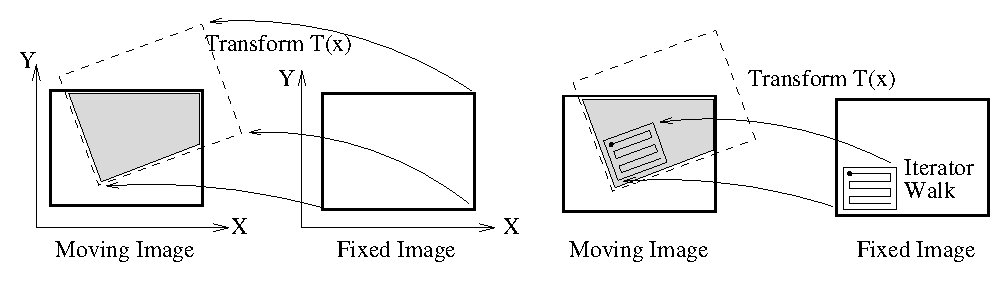
\includegraphics{ImageOverlap.eps}

An Image A is mapped over an image B by using a Transform


\subsection{Iterator Walking over a Region}

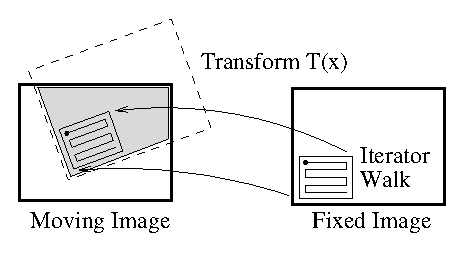
\includegraphics{ImageOverlapIterator.eps} 

An Iterator walking over a region of
B gets mapped on top of a blue region of A

\subsection{Need for an Interpolator}

The positions of the iterator are mapped
on non-grid positions in the image A 

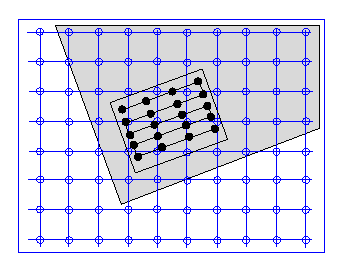
\includegraphics{ImageOverlapInterpolator.eps}

An interpolation is needed for estimating
the value of the image A at these non-grid positions.


\subsection{Overlaped regions }

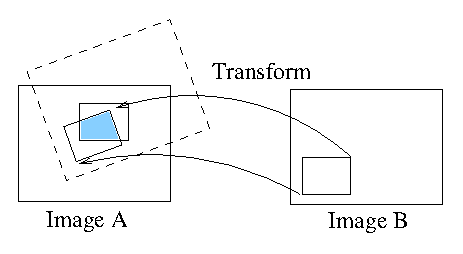
\includegraphics{ImageOverlapedRegions.eps}

Image metrics perform the computation over the intersection of a region in
image A and the map of a region in image B.



\fi

% the clearpage command helps to avoid orphans in the title of the next
% section.
\clearpage

\section{Metrics}
\label{sec:Metrics}
\ifitkFullVersion
%
%  This file is included by Registration.tex
%
%
%

\index{itk::Image\-To\-Image\-Metricv4}

In ITK, \doxygen{ImageToImageMetricv4} objects quantitatively measure how well
the transformed moving image fits the fixed image by comparing the gray-scale
intensity of the images. These metrics are very flexible and can work with any
transform or interpolation method and do not require reduction of the
gray-scale images to sparse extracted information such as edges.

The metric component is perhaps the most critical element of the registration
framework. The selection of which metric to use is highly dependent on the
registration problem to be solved. For example, some metrics have a large
capture range while others require initialization close to the optimal
position.  In addition, some metrics are only suitable for comparing images
obtained from the same imaging modality, while others can handle
inter-modality comparisons.
Unfortunately, there are no clear-cut rules as to how to choose a metric.

\index{itk::Image\-To\-Image\-Metricv4!GetValue()}
\index{itk::Image\-To\-Image\-Metricv4!GetDerivatives()}
\index{itk::Image\-To\-Image\-Metricv4!GetValueAndDerivatives()}

The matching Metric class controls most parts of the registration process
since it handles fixed, moving and virtual images as well as fixed and moving
transforms and interpolators.  The method \code{GetValue()} can be used to
evaluate the quantitative criterion at the transform parameters specified in
the argument.  Typically, the metric samples points within a defined region
of the virtual lattice.  For each point, the corresponding fixed and moving
image positions are computed using the fixed initial transform and the moving
transform with the specified parameters. Then, the fixed and moving interpolators
are used to compute the fixed and moving image's intensities at the mapped
positions. Details on this mapping are illustrated in Figures
\ref{fig:ImageOverlapIterator} and \ref{fig:ImageOverlapInterpolator} assuming
that virtual lattice is the same as the fixed image lattice, which is usually the
case in practice.

The metrics also support region-based evaluation. The \code{SetFixedImageMask()} and
\code{SetMovingImageMask()} methods may be used to restrict evaluation of the metric
within a specified region. The masks may be of any type derived from \doxygen{SpatialObject}.

Besides the measure value, gradient-based optimization schemes also require
derivatives of the measure with respect to each transform parameter. The
methods \code{GetDerivatives()} and \code{GetValueAndDerivatives()} can be
used to obtain the gradient information.


The following is the list of metrics currently available in ITKv4 registration framework:
\begin{itemize}
\item Mean squares\\ \doxygen{MeanSquaresImageToImageMetricv4}
\item Correlation \\ \doxygen{CorrelationImageToImageMetricv4}
\item Mutual information by Mattes \\ \doxygen{MattesMutualInformationImageToImageMetricv4}
\item Joint histogram mutual information \\ \doxygen{JointHistogramMutualInformationHistogramImageToImageMetricv4}
\item Demons metric \\ \doxygen{DemonsImageToImageMetricv4}
\item ANTS neighborhood correlation metric \\ \doxygen{ANTSNeighborhoodCorrelationImageToImageMetricv4}
\end{itemize}

Also, in case you are interested in using the legacy ITK registration framework,
the following is the list of metrics currently available in ITKv3:
\begin{itemize}
\item Mean squares\\ \doxygen{MeanSquaresImageToImageMetric}
\item Normalized correlation \\ \doxygen{NormalizedCorrelationImageToImageMetric}
\item Mean reciprocal squared difference \\ \doxygen{MeanReciprocalSquareDifferenceImageToImageMetric}
\item Mutual information by Viola and Wells \\ \doxygen{MutualInformationImageToImageMetric}
\item Mutual information by Mattes \\ \doxygen{MattesMutualInformationImageToImageMetric}
\item Kullback Liebler distance metric by Kullback and Liebler \\ \doxygen{KullbackLeiblerCompareHistogramImageToImageMetric}
\item Normalized mutual information \\ \doxygen{NormalizedMutualInformationHistogramImageToImageMetric}
\item Mean squares histogram \\ \doxygen{MeanSquaresHistogramImageToImageMetric}
\item Correlation coefficient histogram \\ \doxygen{CorrelationCoefficientHistogramImageToImageMetric}
\item Cardinality Match metric \\ \doxygen{MatchCardinalityImageToImageMetric}
\item Kappa Statistics metric\\ \doxygen{KappaStatisticImageToImageMetric}
\item Gradient Difference metric \\ \doxygen{GradientDifferenceImageToImageMetric}
\end{itemize}

In the following sections, we describe the ITKv4 metric types in detail.
You can check ITK descriptions in doxygen for details about ITKv3 metric classes.

For ease of notation, we will refer to the fixed image $f(\bf{X})$
and transformed moving image $(m \circ T(\bf{X}))$ as images $A$ and $B$.

\subsection{Mean Squares Metric}
\label{sec:MeanSquaresMetricv4}
\index{itk::Mean\-Squares\-Image\-To\-Image\-Metricv4}

The \doxygen{MeanSquaresImageToImageMetricv4} computes the mean squared
pixel-wise difference in intensity between image $A$ and $B$ over a user
defined region:

\begin{equation}
MS(A,B) = \frac{1}{N} \sum_{i=1}^N \left( A_i - B_i \right)^2
\end{equation}
\begin{center}
$A_i$ is the i-th pixel of Image A\\
$B_i$ is the i-th pixel of Image B\\
$N$ is the number of pixels considered
\end{center}

The optimal value of the metric is zero. Poor matches between images $A$ and
$B$ result in large values of the metric. This metric is simple to compute and
has a relatively large capture radius.

This metric relies on the assumption that intensity representing the same
homologous point must be the same in both images. Hence, its use is restricted
to images of the same modality. Additionally, any linear changes in the
intensity result in a poor match value.

\subsubsection{Exploring a Metric}
\label{sec:ExploringAMetric}

Getting familiar with the characteristics of the Metric as a cost function is
fundamental in order to find the best way of setting up an optimization process
that will use this metric for solving a registration problem. The following
example illustrates a typical mechanism for studying the characteristics of a
Metric. Although the example is using the Mean Squares metric, the same
methodology can be applied to any of the other metrics available in the
toolkit.

\ifitkFullVersion
\input{MeanSquaresImageMetric1.tex}
\fi


\subsection{Normalized Correlation Metric}
\label{sec:NormalizedCorrelationMetric}
\index{itk::Correlation\-Image\-To\-Image\-Metricv4}

The \doxygen{CorrelationImageToImageMetricv4} computes pixel-wise
cross-correlation and normalizes it by the square root of the autocorrelation
of the images:

\begin{equation}
NC(A,B) = -1 \times \frac{ \sum_{i=1}^N \left( A_i \cdot B_i \right) }
        { \sqrt { \sum_{i=1}^N A_i^2  \cdot \sum_{i=1}^N B_i^2 } }
\end{equation}
\begin{center}
$A_i$ is the i-th pixel of Image A\\
$B_i$ is the i-th pixel of Image B\\
$N$ is the number of pixels considered
\end{center}

Note the $-1$ factor in the metric computation. This factor is used to make the
metric be optimal when its minimum is reached.  The optimal value of the metric
is then minus one. Misalignment between the images results in small measure
values.  The use of this metric is limited to images obtained using the same
imaging modality.  The metric is insensitive to multiplicative factors between
the two images.  This metric produces a cost function with sharp peaks and
well-defined minima.  On the other hand, it has a relatively small capture radius.


\subsection{Mutual Information Metric}
\label{sec:MutualInformationMetric}

The \doxygen{MattesMutualInformationImageToImageMetricv4} computes the mutual
information between image $A$ and image $B$.  Mutual information (MI)
measures how much information one random variable (image intensity in one
image) tells about another random variable (image intensity in the other
image). The major advantage of using MI is that the actual form of the
dependency does not have to be specified.  Therefore, complex mapping between
two images can be modeled.  This flexibility makes MI well suited as a
criterion of multi-modality registration~\cite{Pluim2003}.

Mutual information is defined in terms of entropy. Let
\begin{equation}
H(A) = - \int p_A(a) \log p_A(a)\, da
\end{equation}
be the entropy of random variable $A$, $H(B)$ the entropy of
random variable $B$ and
\begin{equation}
H(A,B) = \int p_{AB}(a,b) \log p_{AB}(a,b)\,da\,db
\end{equation}
be the joint entropy of $A$ and $B$. If $A$ and $B$ are independent, then
\begin{equation}
p_{AB}(a,b) = p_A(a) p_B(b)
\end{equation}
and
\begin{equation}
H(A,B) = H(A) + H(B).
\end{equation}
However, if there is any dependency, then
\begin{equation}
H(A,B)<H(A)+H(B).
\end{equation}
The difference is called Mutual Information : \( I(A,B) \)
\begin{equation}
I(A,B)=H(A)+H(B)-H(A,B)
\end{equation}

\subsubsection{Parzen Windowing}


\begin{floatingfigure}[rlp]{0.5\textwidth}
 \centering
 \includegraphics[width=0.48\textwidth]{ParzenWindowing13.eps}
 \caption[Parzen Windowing in Mutual Information]{
In Parzen windowing, a continuous density function is constructed by
superimposing kernel functions (Gaussian function in this case) centered on the
intensity samples obtained from the image.\label{fig:ParzenWindowing}}
\end{floatingfigure}

In a typical registration problem, direct access to the marginal
and joint probability densities is not available and hence the
densities must be estimated from the image data. Parzen windows
(also known as kernel density estimators) can be used for this purpose.
In this scheme, the densities are constructed by taking intensity
samples $S$ from the image and super-positioning kernel functions
$K(\cdot)$ centered on the elements of $S$ as illustrated in
Figure \ref{fig:ParzenWindowing}:

A variety of functions can be used as the smoothing kernel with the
requirement that they are smooth, symmetric, have zero mean and
integrate to one. For example, boxcar, Gaussian and B-spline functions are
suitable candidates.  A smoothing parameter is used to scale the kernel
function.  The larger the smoothing parameter, the wider the kernel function
used and hence the smoother the density estimate. If the parameter is too
large, features such as modes in the density will get smoothed out.  On the
other hand, if the smoothing parameter is too small, the resulting density
may be too noisy. The estimation is given by the following equation.

\begin{equation}
p(a) \approx P^{*}(a) = \frac{1}{N} \sum_{s_j \in S} K\left(a - s_j\right)
\end{equation}

Choosing the optimal smoothing parameter is a difficult research problem and
beyond the scope of this software guide.  Typically, the optimal value of the
smoothing parameter will depend on the data and the number of samples used.

\subsubsection{Mattes et al. Implementation}
The implementation of mutual information metric available in ITKv4 follows
the method specified by Mattes et al. in \cite{Mattes2001} and is implemented
by the \doxygen{MattesMutualInformationImageToImageMetricv4} class.

\index{itk::Mattes\-Mutual\-Information\-Image\-To\-Image\-Metricv4}
In this implementation, only one set of intensity samples is drawn from the
image.  Using this set, the marginal and joint probability density function
(PDF) is evaluated at discrete positions or bins uniformly spread within the
dynamic range of the images. Entropy values are then computed by summing over
the bins.

\index{itk::Mattes\-Mutual\-Information\-Image\-To\-Image\-Metricv4!SetNumberOfHistogramBins()}

The number of spatial samples used is a ratio of the total number of samples
and is set using the \code{SetMetricSamplingPercentage()} method directly from
the registration framework \doxygen{ImageRegistrationMethodv4}. Also, The number
of bins used to compute the entropy values is set in the metric class
via the \code{SetNumberOfHistogramBins()} method.

Since the fixed image PDF does not contribute to the metric derivatives, it
does not need to be smooth. Hence, a zero-order (boxcar) B-spline kernel is
used for computing the PDF. On the other hand, to ensure smoothness, a
third-order B-spline kernel is used to compute the moving image intensity PDF. The
advantage of using a B-spline kernel over a Gaussian kernel is that the
B-spline kernel has a finite support region. This is computationally
attractive, as each intensity sample only affects a small number of bins and
hence does not require a $N \times N$ loop to compute the metric value.

During the PDF calculations, the image intensity values are linearly scaled
to have a minimum of zero and maximum of one. This rescaling means that a
fixed B-spline kernel bandwidth of one can be used to handle image data with
arbitrary magnitude and dynamic range.


\subsection{Normalized Mutual Information Metric}
Given two images, $A$ and $B$, the normalized mutual information may be computed as
\begin{equation}
NMI(A,B) = 1 + \frac{I(A,B)}{H(A,B)} = \frac{H(A) + H(B)}{H(A,B)}
\end{equation}
where the entropy of the images, $H(A)$, $H(B)$, the mutual
information, $I(A,B)$ and the joint entropy $H(A,B)$ are computed as mentioned
in \ref{sec:MutualInformationMetric}. Details of the implementation may be found in
\cite{Hajnal2001}.

\subsection{Demons metric}
\index{itk::Demons\-Image\-To\-Image\-Metricv4}

The implementation of the \doxygen{DemonsImageToImageMetricv4} metric is taken from
\doxygen{DemonsRegistrationFunction}.

The metric derivative can be calculated using image derivatives
either from the fixed or moving images. The default is to use fixed-image
gradients. See ObjectToObjectMetric::SetGradientSource to change
this behavior.

An intensity threshold is used, below which image pixels are considered
equal for the purpose of derivative calculation. The threshold can be
changed by calling \code{SetIntensityDifferenceThreshold}.

Note that this metric supports only moving transforms with local support and
with a number of local parameters that match the moving image dimension.
In particular, it's meant to be used with \doxygen{DisplacementFieldTransform}
and derived classes.


\subsection{ANTS neighborhood correlation metric}
\index{itk::ANTS\-Neighborhood\-Correlation\-Image\-To\-Image\-Metricv4}

The \doxygen{ANTSNeighborhoodCorrelationImageToImageMetricv4} metric computes
normalized cross correlation using a small neighborhood for each voxel between
two images, with speed optimizations for dense registration.

Around each voxel, the neighborhood is defined as a N-Dimensional
rectangle centered at the voxel. The size of the rectangle is 2*radius+1.
Normalized correlation between neighborhoods of the fixed image and the moving
image are averaged over the whole image as the final metric.
A radius less than 2 can be unstable. 2 is the default.

\fi

% the clearpage command helps to avoid orphans in the title of the next
% section.
\clearpage

\section{Optimizers}
\label{sec:Optimizers}
\ifitkFullVersion

\index{itk::ObjectToObjectOptimizer}
\index{itk::Single\-Valued\-NonLinear\-Vnl\-Optimizerv4}


\begin{figure}
\center
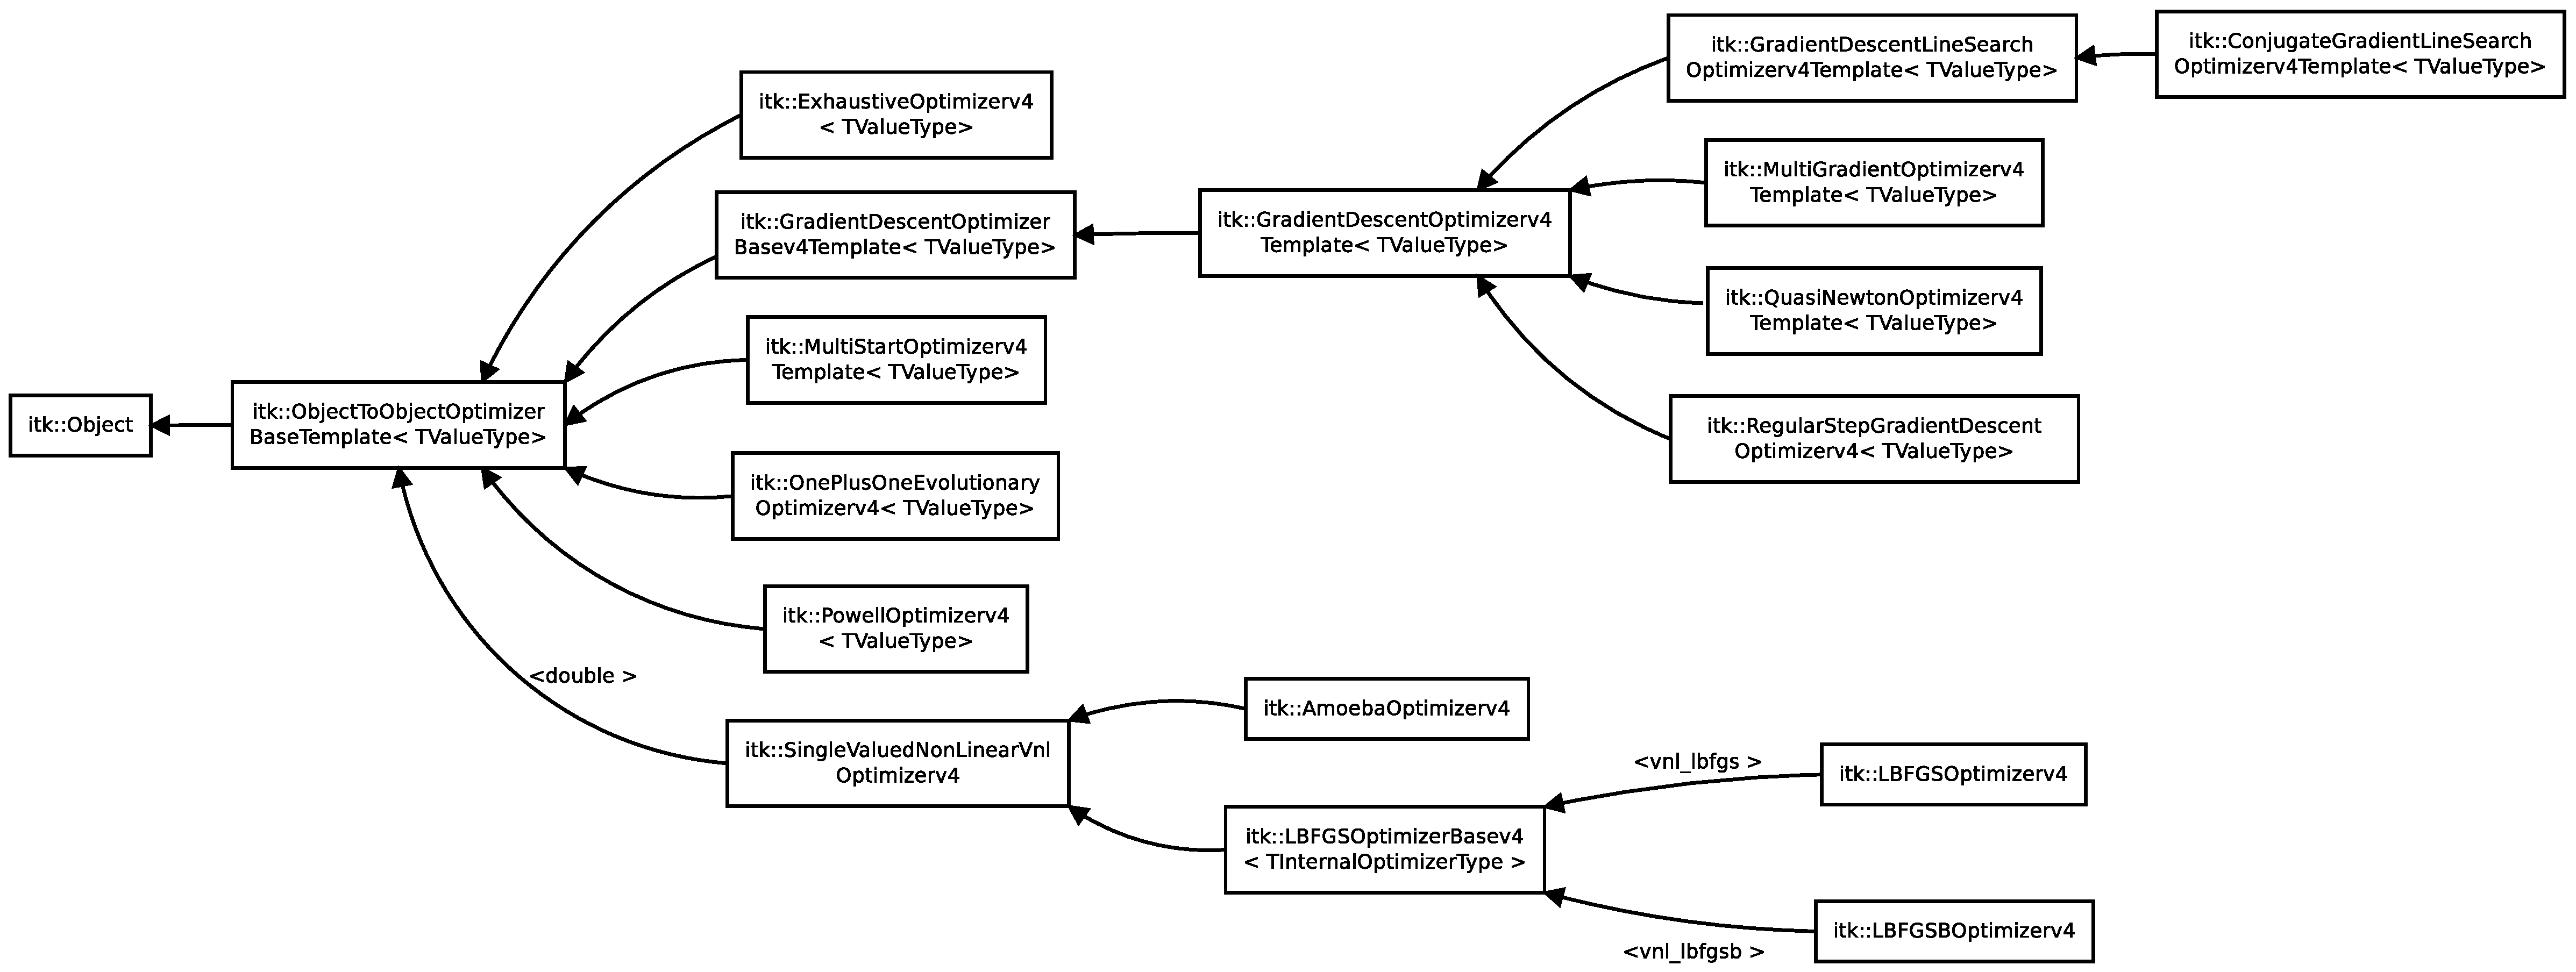
\includegraphics[width=\textheight,angle=90]{Optimizersv4Hierarchy.eps}
\itkcaption[Class diagram of the Optimizers hierarchy in ITKv4]{Class diagram of the
optimizersv4 hierarchy.}
\label{fig:Optimizersv4Hierarchy}
\end{figure}

Optimization algorithms are encapsulated as \doxygen{ObjectToObjectOptimizer}
objects within ITKv4. Optimizers are generic and can be used for applications
other than registration. Within the registration framework, subclasses of
\doxygen{SingleValuedNonLinearVnlOptimizerv4} are implemented as a wrap
around already implemented vnl classes.

\index{itk::ObjectToObjectOptimizer!SetMetric()}
\index{itk::ObjectToObjectOptimizer!StartOptimization()}
\index{itk::ObjectToObjectOptimizer!GetCurrentPosition()}

The basic input to an optimizer is a cost function or metric object. In the context
of registration, \doxygen{ImageToImageMetricv4} classes provide this functionality.
The metric is set using \code{SetInitialPosition()} and
the optimization algorithm is invoked by \code{StartOptimization()}.
Once the optimization has finished, the final parameters can be obtained
using \code{GetCurrentPosition()}.

\index{itk::ObjectToObjectOptimizer!SetScales()}
Some optimizers also allow rescaling of their individual parameters. This is
convenient for normalizing parameter spaces where some parameters have
different dynamic ranges. For example, the first parameter of
\doxygen{Euler2DTransform} represents an angle while the last two parameters
represent translations. A unit change in angle has a much greater impact on an
image than a unit change in translation. This difference in scale appears as
long narrow valleys in the search space making the optimization problem more
difficult. Rescaling the translation parameters can help to fix this problem.
Scales are represented as an \doxygen{Array} of doubles and set using
\code{SetScales()}.

\index{itk::ObjectToObjectOptimizer!SetScalesEstimator()}
Estimating the scales parameters can also be done automatically using the
\doxygen{OptimizerParameterScalesEstimatorTemplate} and its subclasses.
The scales estimator object is then set to the optimizer via
\code{SetScalesEstimator()}.

Despite the old version of ITK, there are only \emph{Single Valued} types
of optimizers available in ITKv4, which are suitable for dealing with cost
functions that return a single value. These are indeed the most common type
of cost functions, and are also known as \emph{Single Valued} functions.

The types of single valued optimizers currently available in ITKv4 are:

\index{itk::Gradient\-Descent\-Optimizerv4}
\index{itk::Regular\-Step\-Gradient\-Descent\-Optimizerv4}
\index{itk::Gradient\-Descent\-Line\-Search\-Optimizerv4}
\index{itk::Conjugate\-Gradient\-Line\-Search\-Optimizerv4}
\index{itk::Multi\-Gradient\-Optimizerv4}
\index{itk::Quasi\-Newton\-Optimizerv4}
\index{itk::Amoeba\-Optimizer}
\index{itk::LBFGS\-Optimizerv4}
\index{itk::LBFGSB\-Optimizerv4}
\index{itk::One\-Plus\-One\-Evolutionary\-Optimizerv4}
\index{itk::Powell\-Optimizerv4}
\index{itk::Exhaustive\-Optimizerv4}


\begin{itemize}

\item \textbf{Amoeba}: Nelder-Meade downhill simplex.  This optimizer is
actually implemented in the \code{vxl/vnl} numerics toolkit.  The ITK class
\doxygen{AmoebaOptimizerv4} is merely an adaptor class.

\item \textbf{Gradient Descent}: Advances parameters in the direction of the
gradient where the step size is governed by a learning rate
(\doxygen{GradientDescentOptimizerv4}).

\item \textbf{Gradient Descent Line Search}: Gradient descent with a golden
section line search. \doxygen{GradientDescentLineSearchOptimizerv4} implements
a simple gradient descent optimizer that is followed by a line search to find
the best value for the learning rate.

\item \textbf{Conjugate Gradient Descent Line Search}: Advances parameters in
the direction of the Polak-Ribiere conjugate gradient where a line search is
used to find the best value for the learning rate
(\doxygen{ConjugateGradientLineSearchOptimizerv4}).

\item \textbf{Quasi Newton}: Implements a Quasi-Newton optimizer with BFGS
Hessian estimation. Second order approximation of the cost function is usually
more efficient since it estimates the descent or ascent direction more precisely.
However, computation of Hessian is usually expensive or unavailable. Alternatively
Quasi-Newton methods can estimate a Hessian from the gradients in previous steps.
Here a specific Quasi-Newton method, BFGS, is used to compute the Quasi-Newton steps
(\doxygen{QuasiNewtonOptimizerv4}).

\item \textbf{LBFGS}: Limited memory Broyden, Fletcher, Goldfarb
and Shannon minimization. It is an adaptor to an optimizer in \code{vnl}
(\doxygen{LBFGSOptimizerv4}).

\item \textbf{LBFGSB}: A modified version of the LBFGS optimizer that allows to
specify bounds for the parameters in the search space.  It is an adaptor to an
optimizer in \code{netlib}. Details on this optimizer can be found
in~\cite{Byrd1995,Zhu1997} (\doxygen{LBFGSBOptimizerv4}).

\item \textbf{One Plus One Evolutionary}: Strategy that simulates the
biological evolution of a set of samples in the search space. This optimizer is
mainly used in the process of bias correction of MRI images
(\doxygen{OnePlusOneEvolutionaryOptimizerv4}). Details on this optimizer can be
found in~\cite{Styner2000}.

\item \textbf{Regular Step Gradient Descent}: Advances parameters in the
direction of the gradient where a bipartition scheme is used to compute
the step size (\doxygen{RegularStepGradientDescentOptimizerv4}).
This optimizer is also used for Versor transforms parameters, where the
current rotation is composed with the gradient rotation to produce the
new rotation versor. The translational part of the transform parameters
are updated as usually done in a vector space. It follows the definition
of versor gradients defined by Hamilton~\cite{Hamilton1866}

\item \textbf{Powell Optimizer}: Powell optimization method.  For an
N-dimensional parameter space, each iteration minimizes(maximizes) the function
in N (initially orthogonal) directions. This optimizer is described
in~\cite{Press1992}.  (\doxygen{PowellOptimizerv4}).

\item \textbf{Exhausive Optimizer}: Fully samples a grid on the parameteric space.
This optimizer is equivalent to an exahaustive search in a discrete grid defined
over the parametric space. The grid is centered on the initial position. The
subdivisions of the grid along each one of the dimensions of the parametric space
is defined by an array of number of steps
(\doxygen{ExhaustiveOptimizerv4}).

\end{itemize}

Figure \ref{fig:Optimizersv4Hierarchy} illustrates the full class hierarchy of
optimizers in ITK. Optimizers in the lower right corner are adaptor classes
to optimizers existing in the \code{vxl/vnl} numerics toolkit. The optimizers
interact with the \doxygen{CostFunction} class. In the registration framework
this cost function is reimplemented in the form of ImageToImageMetric.






\fi



\subsection{Registration using Match Cardinality metric}
\label{sec:RegistrationMatchCardinality}
\ifitkFullVersion
\input{ImageRegistration10.tex}
\fi


\subsection{Registration using the One plus One Evolutionary Optimizer}
\label{sec:RegistrationOnePlusOne}
\ifitkFullVersion
\input{ImageRegistration11.tex}
\fi



\subsection{Registration using masks constructed with Spatial objects}
\label{sec:RegistrationSpatialObjects}
\ifitkFullVersion
\input{ImageRegistration12.tex}
\fi



\subsection{Rigid registrations incorporating prior knowledge}
\label{sec:RegistrationCentered2DTransform}
\ifitkFullVersion
\input{ImageRegistration13.tex}
\fi
% the clearpage command helps to avoid orphans in the title of the next
% section.
\clearpage

\section{Image Pyramids}
\label{sec:ImagePyramids}
\ifitkFullVersion

\index{itk::MultiResolutionPyramidImageFilter|textbf}

In ITK, the \code{MultiResolutionPyramidImageFilter} can be used to create a
sequence of down-sampled version of the input image.  The down-sampling is done
according to a user defined multi-resolution schedule. The schedule is
specified as an \code{Array2D<int>} containing shrink factors for each
multi-resolution level (rows) for each dimension (columns). For example,

\begin{verbatim}
8 4 4
4 4 2
\end{verbatim}

is a schedule for a three dimensional image for two multi-resolution levels. 
In the first (coarsest) level, the image is reduced by a factor of 8 
in the column dimension, factor of 4 in the row dimension and a factor
of 4 in the slice dimension. In the second level, the image reduced
by a factor of 4 in the column dimension, 4 in the row dimension and
2 in the slice dimension.

\index{itk::MultiResolutionPyramidImageFilter!SetNumberOfLevels()}

The method \code{SetNumberOfLevels()} is used to set the number of
resolution levels in the pyramid. This method will allocate memory
for the schedule and generates a default table with the starting
(coarsest) shrink factors for all dimension set to $(M-1)^2$, 
where $M$ is the number of levels. All factors are halved for
all subsequent levels. For example, if we set the number of levels
to 4, the default schedule is then:

\begin{verbatim}
8 8 8
4 4 4
2 2 2
1 1 1
\end{verbatim}

\index{itk::MultiResolutionPyramidImageFilter!GetSchedule()}
\index{itk::MultiResolutionPyramidImageFilter!SetSchedule()}
\index{itk::MultiResolutionPyramidImageFilter!SetStartingShrinkFactors()}

The user can get a copy of the schedule using method \code{GetSchedule()},
make modifications and reset it using method \code{SetSchedule()}.
Alternatively, a user can create a default table by specifying the
starting (coarsest) shrink factors using method 
\code{SetStartingShrinkFactors()}. The factors for the subsequent
levels are generated by halving the factor or setting to one, 
depending on which is larger. For example, for a 4 level pyramid
and starting factors of 8, 8 and 4, the generated schedule would be:

\begin{verbatim}
8 8 4
4 4 2
2 2 1
1 1 1
\end{verbatim}

When this filter is triggered by \code{Update()}, $M$ outputs are produced
where the $m$-th output correspond to the $m$-th level of the pyramid.
To generate these images, Gaussian smoothing is first performed using a
\code{DiscreteGaussianImageFilter} with the variance set to $(s/2)^2$,
where $s$ is the shrink factor. The smoothed images are then sub-sampled using
a \code{ShrinkImageFilter}.

\fi


% the clearpage command helps to avoid orphans in the title of the next
% section.
\clearpage

\section{Deformable Registration}
\label{sec:DeformableRegistration}
\ifitkFullVersion
%%%%%%%%%%%%%%%%%%%%%%%%%%%%%%%%%%%%%%%%%%%%%%%%%%%%%%%%%%%%%%%
%
%
%   This file is included in Registration.tex
%
%   Lablels and section entries are defined in that file.
%
%
%
%%%%%%%%%%%%%%%%%%%%%%%%%%%%%%%%%%%%%%%%%%%%%%%%%%%%%%%%%%%%%%%

 
\begin{figure} \center
\includegraphics[width=0.44\textwidth]{DeformableRegistration1CheckerboardBefore.eps}
\includegraphics[width=0.44\textwidth]{DeformableRegistration1CheckerboardAfter.eps}
\itkcaption[FEM-based deformable registration results]{Checkerboard comparisons
before and after FEM-based deformable registration.}
\label{fig:DeformableRegistration1Output}
\end{figure}

\ifitkFullVersion
\input{DeformableRegistration1.tex}
\fi

Figure \ref{fig:DeformableRegistration1Output} presents the results of
the FEM-based deformable registration applied to two time-separated
slices of a living mouse dataset.  Checkerboard comparisons of the two
images are shown before registration (left) and after registration
(right).  Both images were acquired from the same living mouse, the
first after inspiration of air into the lungs and the second after
exhalation.  Deformation occurs due to the elastic recoil of the lung
tissue and the relaxation of the diaphragm.

The following is a documented sample parameter file that can be used with this
deformable registration example.  This example demonstrates the setup of a
basic registration problem that does not use multi-resolution strategies.  As a
result, only one value for the parameters between \texttt{(\# of pixels per
element)} and \texttt{(maximum iterations)} is necessary.  In order to use a
multi-resolution strategy, you would have to specify values for those
parameters at each level of the pyramid.

\small
\verbatiminput{FiniteElementRegistrationParameters1.txt}
\normalsize



\fi

% the clearpage command helps to avoid orphans in the title of the next
% section.
\clearpage

\section{Demons Deformable Registration}
\label{sec:DemonsDeformableRegistration}
\ifitkFullVersion
%%%%%%%%%%%%%%%%%%%%%%%%%%%%%%%%%%%%%%%%%%%%%%%%%%%%%%%%%%%%%%%
%
%
%   This file is included in Registration.tex
%
%   Lablels and section entries are defined in that file.
%
%
%
%%%%%%%%%%%%%%%%%%%%%%%%%%%%%%%%%%%%%%%%%%%%%%%%%%%%%%%%%%%%%%%

% Brief description of the demons algorithm goes here

\input{DeformableRegistration2.tex} 


\fi

\section{Visualizing Deformation fields}
\label{sec:VisualizingDeformationFields}
\ifitkFullVersion
%%%%%%%%%%%%%%%%%%%%%%%%%%%%%%%%%%%%%%%%%%%%%%%%%%%%%%%%%%%%%%%
%
%
%   This file is included in Registration.tex
%
%   Lablels and section entries are defined in that file.
%
%
%
%%%%%%%%%%%%%%%%%%%%%%%%%%%%%%%%%%%%%%%%%%%%%%%%%%%%%%%%%%%%%%
Vector deformation fields may be visualized using ParaView.
ParaView \cite{ParaviewBook} is an open-source, multi-platform visualization application and uses the Visualization Toolkit as the data processing and rendering engine and has a user interface written using a unique blend of Tcl/Tk and C++. You may download it from http://paraview.org.

\subsection{Visualizing 2D deformation fields}
Let us visualize the deformation field obtained from Demons Registration algorithm generated from ITK/Examples/RegistrationITKv4/DeformableRegistration2.cxx.

Load the Deformation field in Paraview. (The deformation field must be capable of handling vector data, such as MetaImages). Paraview shows a color map of the magnitudes of the deformation fields as shown in \ref{fig:ParaviewScreenshot1}.

Covert the deformation field to 3D vector data using a {\it Calculator}. The Calculator may be found in the {\it Filter} pull down menu. A screenshot of the calculator tab is shown in Figure \ref{fig:ParaviewScreenshot2}. Although the deformation field is a 2D vector, we will generate a 3D vector with the third component set to 0 since Paraview generates glyphs only for 3D vectors. You may now apply a glyph of arrows to the resulting 3D vector field by using {\it Glyph} on the menu bar. The glyphs obtained will be very dense since a glyph is generated for each point in the data set. To better visualize the deformation field, you may adopt one of the following approaches.

Reduce the number of glyphs by reducing the number in {\it Max. Number of Glyphs} to reasonable amount. This uniformly downsamples the number of glyphs. Alternatively, you may apply a {\it Threshold} filter to the {\it Magnitude} of the vector dataset and then glyph the vector data that lies above the threshold. This eliminates the smaller deformation fields that clutter the display. You may now reduce the number of glyphs to a reasonable value.

Figure \ref{fig:ParaviewScreenshot3} shows the vector field visualized using Paraview by thresholding the vector magnitudes by 2.1 and restricting the number of glyphs to 100.

\begin{figure}
\center
\includegraphics[width=\textwidth]{ParaviewScreenshot1.eps}
\itkcaption[Deformation field magnitudes]{Deformation field magnitudes displayed using Paraview}
\label{fig:ParaviewScreenshot1}
\end{figure}

\begin{figure}
\center
\includegraphics[width=0.3\textwidth]{ParaviewScreenshot2.eps}
\itkcaption[Calculator]{Calculators and filters may be used to compute the vector magnitude, compose vectors etc.}
\label{fig:ParaviewScreenshot2}
\end{figure}

\begin{figure}
\center
\includegraphics[width=\textwidth]{ParaviewScreenshot3.eps}
\itkcaption[Visualized Def field]{Deformation field visualized using Paraview after thresholding and subsampling.}
\label{fig:ParaviewScreenshot3}
\end{figure}



\subsection{Visualizing 3D deformation fields}
Let us create a 3D deformation field. We will use Thin Plate Splines to warp a 3D dataset and create a deformation field. We will pick a set of point landmarks and translate them to provide a specification of correspondences at point landmarks. Note that the landmarks have been picked randomly for purposes of illustration and are not intended to portray a true deformation. The landmarks may be used to produce a deformation field in several ways. Most techniques minimize some regularizing functional representing the irregularity of the deformation field, which is usually some function of the spatial derivatives of the field. Here will we use {\it thin plate splines}. Thin plate splines minimize the regularizing functional

\begin{equation}
I[f(x,y)] = \iint (f^2_{xx} + 2 f^2_{xy} + f^2_{yy}) dx dy
\end{equation}
where the subscripts denote partial derivatives of f.

The code for this section can be found in ITK/Examples/RegistrationITKv4/ThinPlateSplineWarp.cxx

We may now proceed as before to visualize the deformation field using Paraview as shown in Figure \ref{fig:ParaviewScreenshot4}.

\begin{figure}
\center
\includegraphics[width=0.7\textwidth]{ParaviewScreenshot4.eps}
\itkcaption[Visualized Def field4]{3D Deformation field visualized using Paraview.}
\label{fig:ParaviewScreenshot4}
\end{figure}




\fi

\ifitkFullVersion
%%%%%%%%%%%%%%%%%%%%%%%%%%%%%%%%%%%%%%%%%%%%%%%%%%%%%%%%%%%%%%%
%
%
%   This file is included in DeformableRegistration.tex
%
%   Lablels and section entries are defined in that file.
%
%
%
%%%%%%%%%%%%%%%%%%%%%%%%%%%%%%%%%%%%%%%%%%%%%%%%%%%%%%%%%%%%%%
Let us register the deformed volumes generated by Thin plate warping in the
previous example using DeformableRegistration4.cxx. Since ITK is in general
N-dimensional, the only change in the example is to replace the
\code{ImageDimension} by 3.

The registration method uses B-splines and an LBFGS optimizer. The trace in
Table. \ref{tab:LBFGStrace} prints the trace of the optimizer through the
search space.

\begin{table}
\begin{center}
\begin{tabular}{\tableconfiguration}
\hline
\textbf{Iteration} &
\textbf{Function value} &
\textbf{$\|G\|$} &
\textbf{Step length} \\
\hline\hline
   1    &        156.981  &    14.911  & 0.202 \\
   2    &        68.956    &    11.774    &    1.500 \\
   3    &        38.146    &    4.802     &   1.500 \\
   4    &        26.690    &    2.515     &   1.500 \\
   5    &        23.295    &    1.106     &   1.500\\
   6    &        21.454    &    1.032     &   1.500\\
   7    &        20.322    &    1.557     &   1.500\\
   8    &        19.751    &    0.594     &   1.500\\
\hline
\end{tabular}
\end{center}
\itkcaption[LBFGS Optimizer trace]{LBFGS Optimizer trace.
\label{tab:LBFGStrace}}
\end{table}

Here $\|G\|$ is the norm of the gradient at the current estimate of the
minimum, $x$. ``Function Value" is the current value of the function, f(x).

The resulting deformation field that maps the moving to the fixed image is
shown in \ref{fig:DeformationFieldOutput}. A difference image of two slices
before and after registration is shown in
\ref{fig:DefRegistrationDiffScreenshot}. As can be seen from the figures, the
deformation field is in close agreement to the one generated from the Thin
plate spline warping.

\begin{figure}
\center
\includegraphics[width=0.6\textwidth]{ParaviewScreenshot5.eps}
\itkcaption[Deformation field output]{Resulting deformation field that maps the moving image to the fixed image.}
\label{fig:DeformationFieldOutput}
\end{figure}

\begin{figure}
\center
\includegraphics[width=0.44\textwidth]{DeformableRegistration4DiffBefore.eps}
\includegraphics[width=0.44\textwidth]{DeformableRegistration4DiffAfter.eps}
\itkcaption[Difference image]{Difference image from a slice before and after registration.}
\label{fig:DefRegistrationDiffScreenshot}
\end{figure}



\fi


% the clearpage command helps to avoid orphans in the title of the next
% section.
\clearpage

\section{Model Based Registration}
\label{sec:ModelBasedRegistration}
\ifitkFullVersion
%%%%%%%%%%%%%%%%%%%%%%%%%%%%%%%%%%%%%%%%%%%%%%%%%%%%%%%%%%%%%%%
%
%
%   This file is included in Registration.tex
%
%   Lablels and section entries are defined in that file.
%
%
%
%%%%%%%%%%%%%%%%%%%%%%%%%%%%%%%%%%%%%%%%%%%%%%%%%%%%%%%%%%%%%%%

\begin{floatingfigure}[rlp]{8cm}
  \centering
  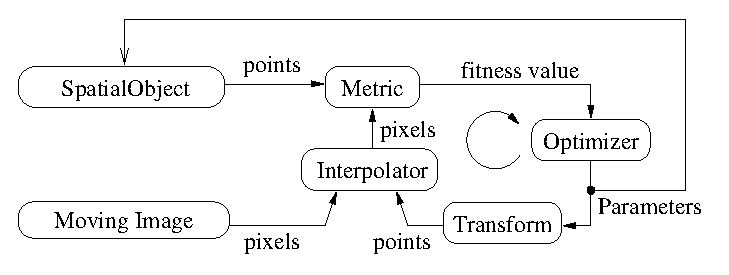
\includegraphics[width=7.5cm]{ModelToImageRegistrationComponentsDiagram.eps}
  \caption[Model to Image Registration Framework Components]{The basic
components of model based registration are an image, a spatial object, a
transform, a metric, an interpolator and an
optimizer.\label{fig:ModelToImageRegistrationComponentsDiagram}}
\end{floatingfigure}

This section introduces the concept of registering a geometrical model with
an image. We refer to this concept as \emph{model based registration} but
this may not be the most widespread terminology. In this approach, a
geometrical model is built first and a number of parameters are identified in
the model. Variations of these parameters make it possible to adapt the model
to the morphology of a particular patient. The task of registration
is then to find the optimal combination of model parameters that will
make this model a good representation of the anatomical structures
contained in an image.

For example, let's say that in the axial view of a brain image we can roughly
approximate the skull with an ellipse. The ellipse becomes our simplified
geometrical model, and registration is the task of finding the best center for
the ellipse, the measures of its axis lengths and its orientation in the plane.
This is illustrated in Figure~\ref{fig:ModelToImageRegistrationConcept}.  If we
compare this approach with the image-to-image registration problem, we can see
that the main difference here is that in addition to mapping the spatial
position of the model, we can also customize internal parameters that change
its shape.

Figure~\ref{fig:ModelToImageRegistrationComponentsDiagram}   illustrates  the
major  components of  the registration  framework in  ITK when  a  model-based
registration problem is configured. The basic input data for the registration
is  provided by  pixel data  in an  \doxygen{Image} and  by  geometrical data
stored in a  \doxygen{SpatialObject}. A metric has to be  defined in order to
evaluate the fitness between the model  and the image. This fitness value can
be  improved by  introducing variations  in  the spatial  positioning of  the
SpatialObject and/or  by changing its  internal parameters. The  search space
for the optimizer  is now the composition of the  transform parameter and the
shape internal parameters.

This same approach can be considered a segmentation technique, since once the
model has been optimally superimposed on the image we could label pixels
according to their associations with specific parts of the model. The
applications of model to image registration/segmentation are endless.
The main advantage of this approach is probably that, as opposed to image-to-image
registration, it actually provides \emph{Insight} into the anatomical structure
contained in the image. The adapted model becomes a condensed representation of
the essential elements of the anatomical structure.

\begin{figure}
\center
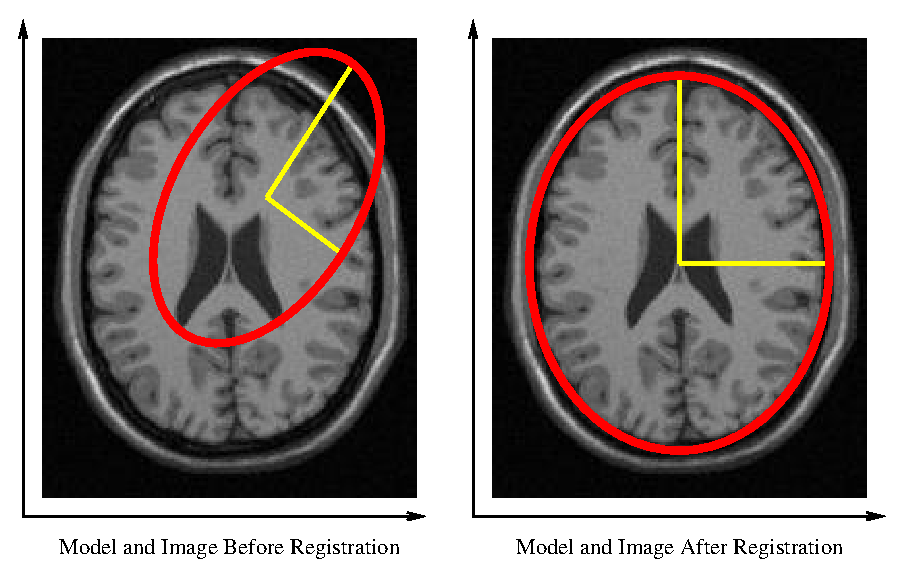
\includegraphics[width=0.8\textwidth]{ModelToImageRegistrationConcept.eps}
\itkcaption[Model to Image Registration Framework Concept]{Basic concept of
  Model-to-Image registration.  A simplified geometrical model (ellipse) is
    registered against an anatomical structure (skull)  by applying a spatial
    transform and modifying the model internal parameters. This image is not
    the result of an actual registration, it is shown here only with the
    purpose of illustrating the concept of model to image registration.}
\label{fig:ModelToImageRegistrationConcept}
\end{figure}


ITK provides a hierarchy of classes intended to support the construction of
shape models. This hierarchy has the SpatialObject as its base class.
A number of basic functionalities are defined at this level, including the
capacity to evaluate whether a given point is \emph{inside} or \emph{outside} of the
model, form complex shapes by creating hierarchical
conglomerates of basic shapes, and support basic spatial
parameterizations like scale, orientation and position.

The following sections present examples of the typical uses of these powerful
elements of the toolkit.

\ifitkFullVersion
\input{ModelToImageRegistration1.tex}
\fi





\fi


\section{Point Set Registration}
\label{sec:PointSetRegistration}

The classical algorithm for performing PointSet to PointSet registration is the
Iterative Closest Point (ICP) algorithm.  The following examples illustrate how
this 0 can be used in ITK.

\ifitkFullVersion
\input{IterativeClosestPoint1.tex}
\fi

\ifitkFullVersion
\input{IterativeClosestPoint2.tex}
\fi

\ifitkFullVersion
\input{IterativeClosestPoint3.tex}
\fi


